%!TEX root = ../thesis.tex

\chapter{Umsetzung}
\label{chap:umsetzung}

Im Folgenden wird die Konzeption und Umsetzung der in \ref{sec:anforderungsanalyse}
beschriebenen Anforderungen an das Projekt \projectname{} erläutert.
Der Schwerpunkt liegt dabei speziell auf der plattformübergreifenden Architektur sowie auf der
Entwicklung der Komponenten hinsichtlich Wiederverwendbarkeit.


\section{Applikationsstruktur}

Dieses Kapitel beschäftigt sich mit der Konzeptphase der plattformübergreifenden Applikationsstruktur
(Abbildung \ref{kapitel4/arch}).
Um Endprodukte für Web, Desktop und App zu generieren, werden die Frameworks Angular 2, Electron und das
Ionic \ac{SDK} verwendet. Die Codebase für die Web- und Desktop-Anwendungen lassen sich so weit vereinen,
dass diese innerhalb eines Repositories implementiert werden können.
Ein weiteres Repository beinhaltet die hybride Applikation,
welche mithilfe des Ionic 2 \ac{SDK} entwickelt wird. Obwohl Ionic 2 auf das Angular Framework aufbaut,
ergibt es Sinn den Web und App Code voneinander getrennt zu behandeln.
Gründe dafür sind zum einen konzeptionelle Unterschiede im Aufbau der Applikationen
sowie Unterschiede in der Grundstruktur der beiden Frameworks.
Die \ac{UI} und Funktionalität wird daher innerhalb der Angular 2
Anwendung in Form von wiederverwendbaren Komponenten entwickelt und
Repository-übergreifend für die Verwendung im Ionic 2 Projekt verteilt.

\begin{itemize}
  \item Angular 2/Web und Desktop: github.com/michaelknoch/mia
  \item Ionic 2/App: github.com/michaelknoch/miamobile
\end{itemize}



\begin{figure}[htbp]
 \centering
 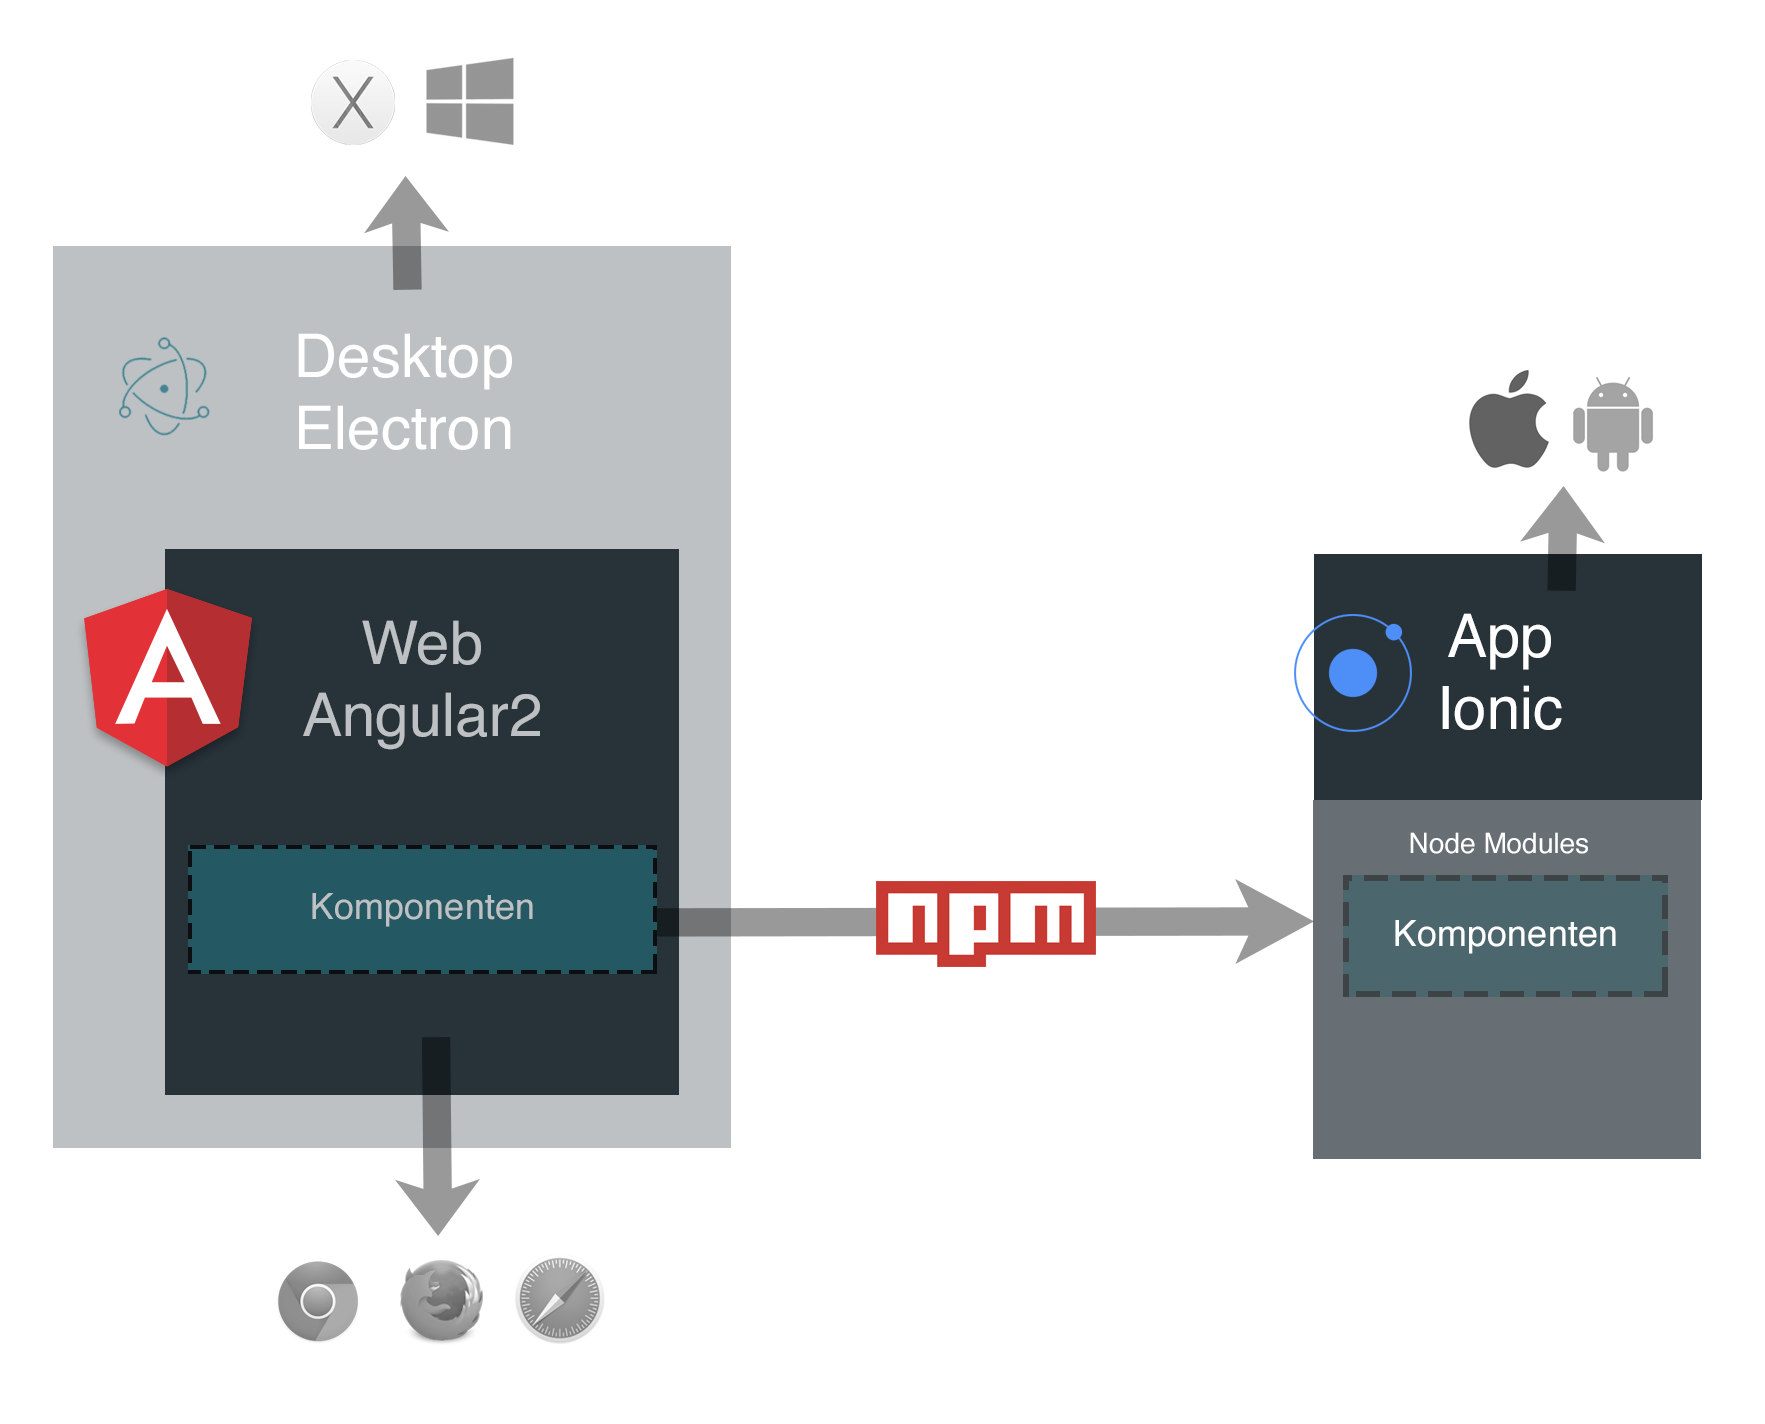
\includegraphics[width=0.55\linewidth]{kapitel4/arch.png}
 \caption{Plattformübergreifende Architektur}
 \label{kapitel4/arch}
\end{figure}




\section{Komponentenentwicklung}

\subsection{Komponententypen}

Im Folgenden werden Ansätze der Komponentenentwicklung bezüglich der in
\projectname{} erforderlichen Funktionalitäten entwickelt.


\subsubsection{Generischer Ansatz}

Bei der Entwicklung generischer Komponenten ist der Begriff der Wiederverwendbarkeit von zentraler Bedeutung.
Komponenten werden gegenüber dem spezifischen Ansatz nicht für einen definierten Anwendungsfall konzipiert,
sondern können
für diverse, womöglich ähnliche Anwendungsbereiche genutzt werden.
Typisch für generische Angular 2 Komponenten ist die Verwendung des Input Kanals.
Dabei werden zum einen Daten- sowie Konfigurationsobjekte von außen in die Komponente eingeschleust.
Anhand der Konfigurationsobjekte können generische Komponenten individuell an verschiedene Bedürfnisse angepasst werden.
Durch den Transfer von Datenobjekten werden Aggregationsvorgänge aus den Komponenten abstrahiert und damit eventuelle
Abhängigkeiten zu Services oder API-Servern vermieden.

Komponenten,
die anhand des generischen Ansatzes entwickelt werden,
sollen nicht ausschließlich in der mobilen App,
sondern projektübergreifend in der Open Source Community Verwendung finden.
Daher wurde ein Teil der in \projectname{} entwickelten Komponenten anhand des generischen Ansatzes
entwickelt und open source auf Github veröffentlicht.
Dadurch können diese von der Community genutzt und bei Bedarf verbessert und um Funktionalität erweitert werden.


\subsubsection{Spezifischer Ansatz}

Einige Komponenten lassen sich aufgrund ihrer spezifischen Funktionalität nicht generisch entwickeln.
Da sie nur einen spezifischen Anwendungsfall abdecken, können sie nur schwer in anderen Projekten wiederverwendet werden.
Dennoch werden diese innerhalb des Projekts \projectname{}
in der Angular 2 sowie in der Ionic 2 Anwendung verwendet.
Beispiele für spezifische Komponenten sind View- und Menükomponenten welche die Grundstruktur der Applikation abbilden.

\subsection{MVC und Abhängigkeiten}

Im Idealfall können Komponenten voneinander gekapselt entwickelt werden,
sodass sie völlig eigenständig nutzbar sind und untereinander keine Abhängigkeiten aufweisen.
Jede Komponente beinhaltet individuelle \ac{MVC} Schichten für die Implementierung der Funktionalität von der View bis zur Datenschicht.
Modelklassen und Services befinden sich innerhalb der Komponente und nicht innerhalb eines globalen Model Layers.
Allerdings entstehen im Aufbau einer Angular Applikation schnell komponentenübergreifende Abhängigkeiten.
Wird Funktionalität in Services, welche von mehreren Komponenten genutzt wird, implementiert,
so sollte diese nicht in die Komponente gekapselt werden, sondern sich in einer sichtbaren Schicht befinden.
Es liegt nahe, dass Typescript Modelklassen ebenfalls in mehreren Komponenten verwendet werden.
Demnach sollten diese nicht redundant implementiert,
sondern zentral zur Verfügung gestellt werden. Es stellt sich heraus,
dass nicht alle Komponenten der Applikation \projectname{} als eigenständige Module ausgeliefert werden können,
sondern es durchaus Sinn ergibt, Komponenten, Service- und Modelklassen anhand ihrer Abhängigkeiten in Paketen zu verwalten und
gebündelt über die Infrastruktur zu verteilen.


\subsection{Komponenten Generator}

Um den Entwicklungsprozess der Komponenten zu beschleunigen, wurde mithilfe von \emph{yeoman.io} ein Komponenten-Generator entwickelt.
Dieser ermöglicht es die Grundstruktur neuer Komponenten anhand diverser Optionen in kurzer Zeit auszuliefern.
Dabei wird der Name sowie der Auslieferungsort der neuen Komponente während der Generierung im Terminal erfragt.
Zusätzlich kann definiert werden, ob externe \ac{HTML} und \ac{CSS} Dateien angelegt, oder ob diese inline in der Komponente definiert werden sollen.
Der Generator wurde ebenfalls open source entwickelt und auf Github veröffentlicht.

\begin{itemize}
\item github.com/michaelknoch/generator-ng2-comp
\end{itemize}


\subsection{Implementierung}

Im Folgenden werden für die Thesis relevante Implementierungen von Komponenten erläutert.
Der zugehörige Anwendungscode befindet sich dabei entweder direkt innerhalb der Beschreibung oder im Anhang dieser Arbeit.

\subsubsection{Login und Authentifizierung}
\label{Login-und-Authentifikation}

\begin{figure}[hptb]
 \centering
 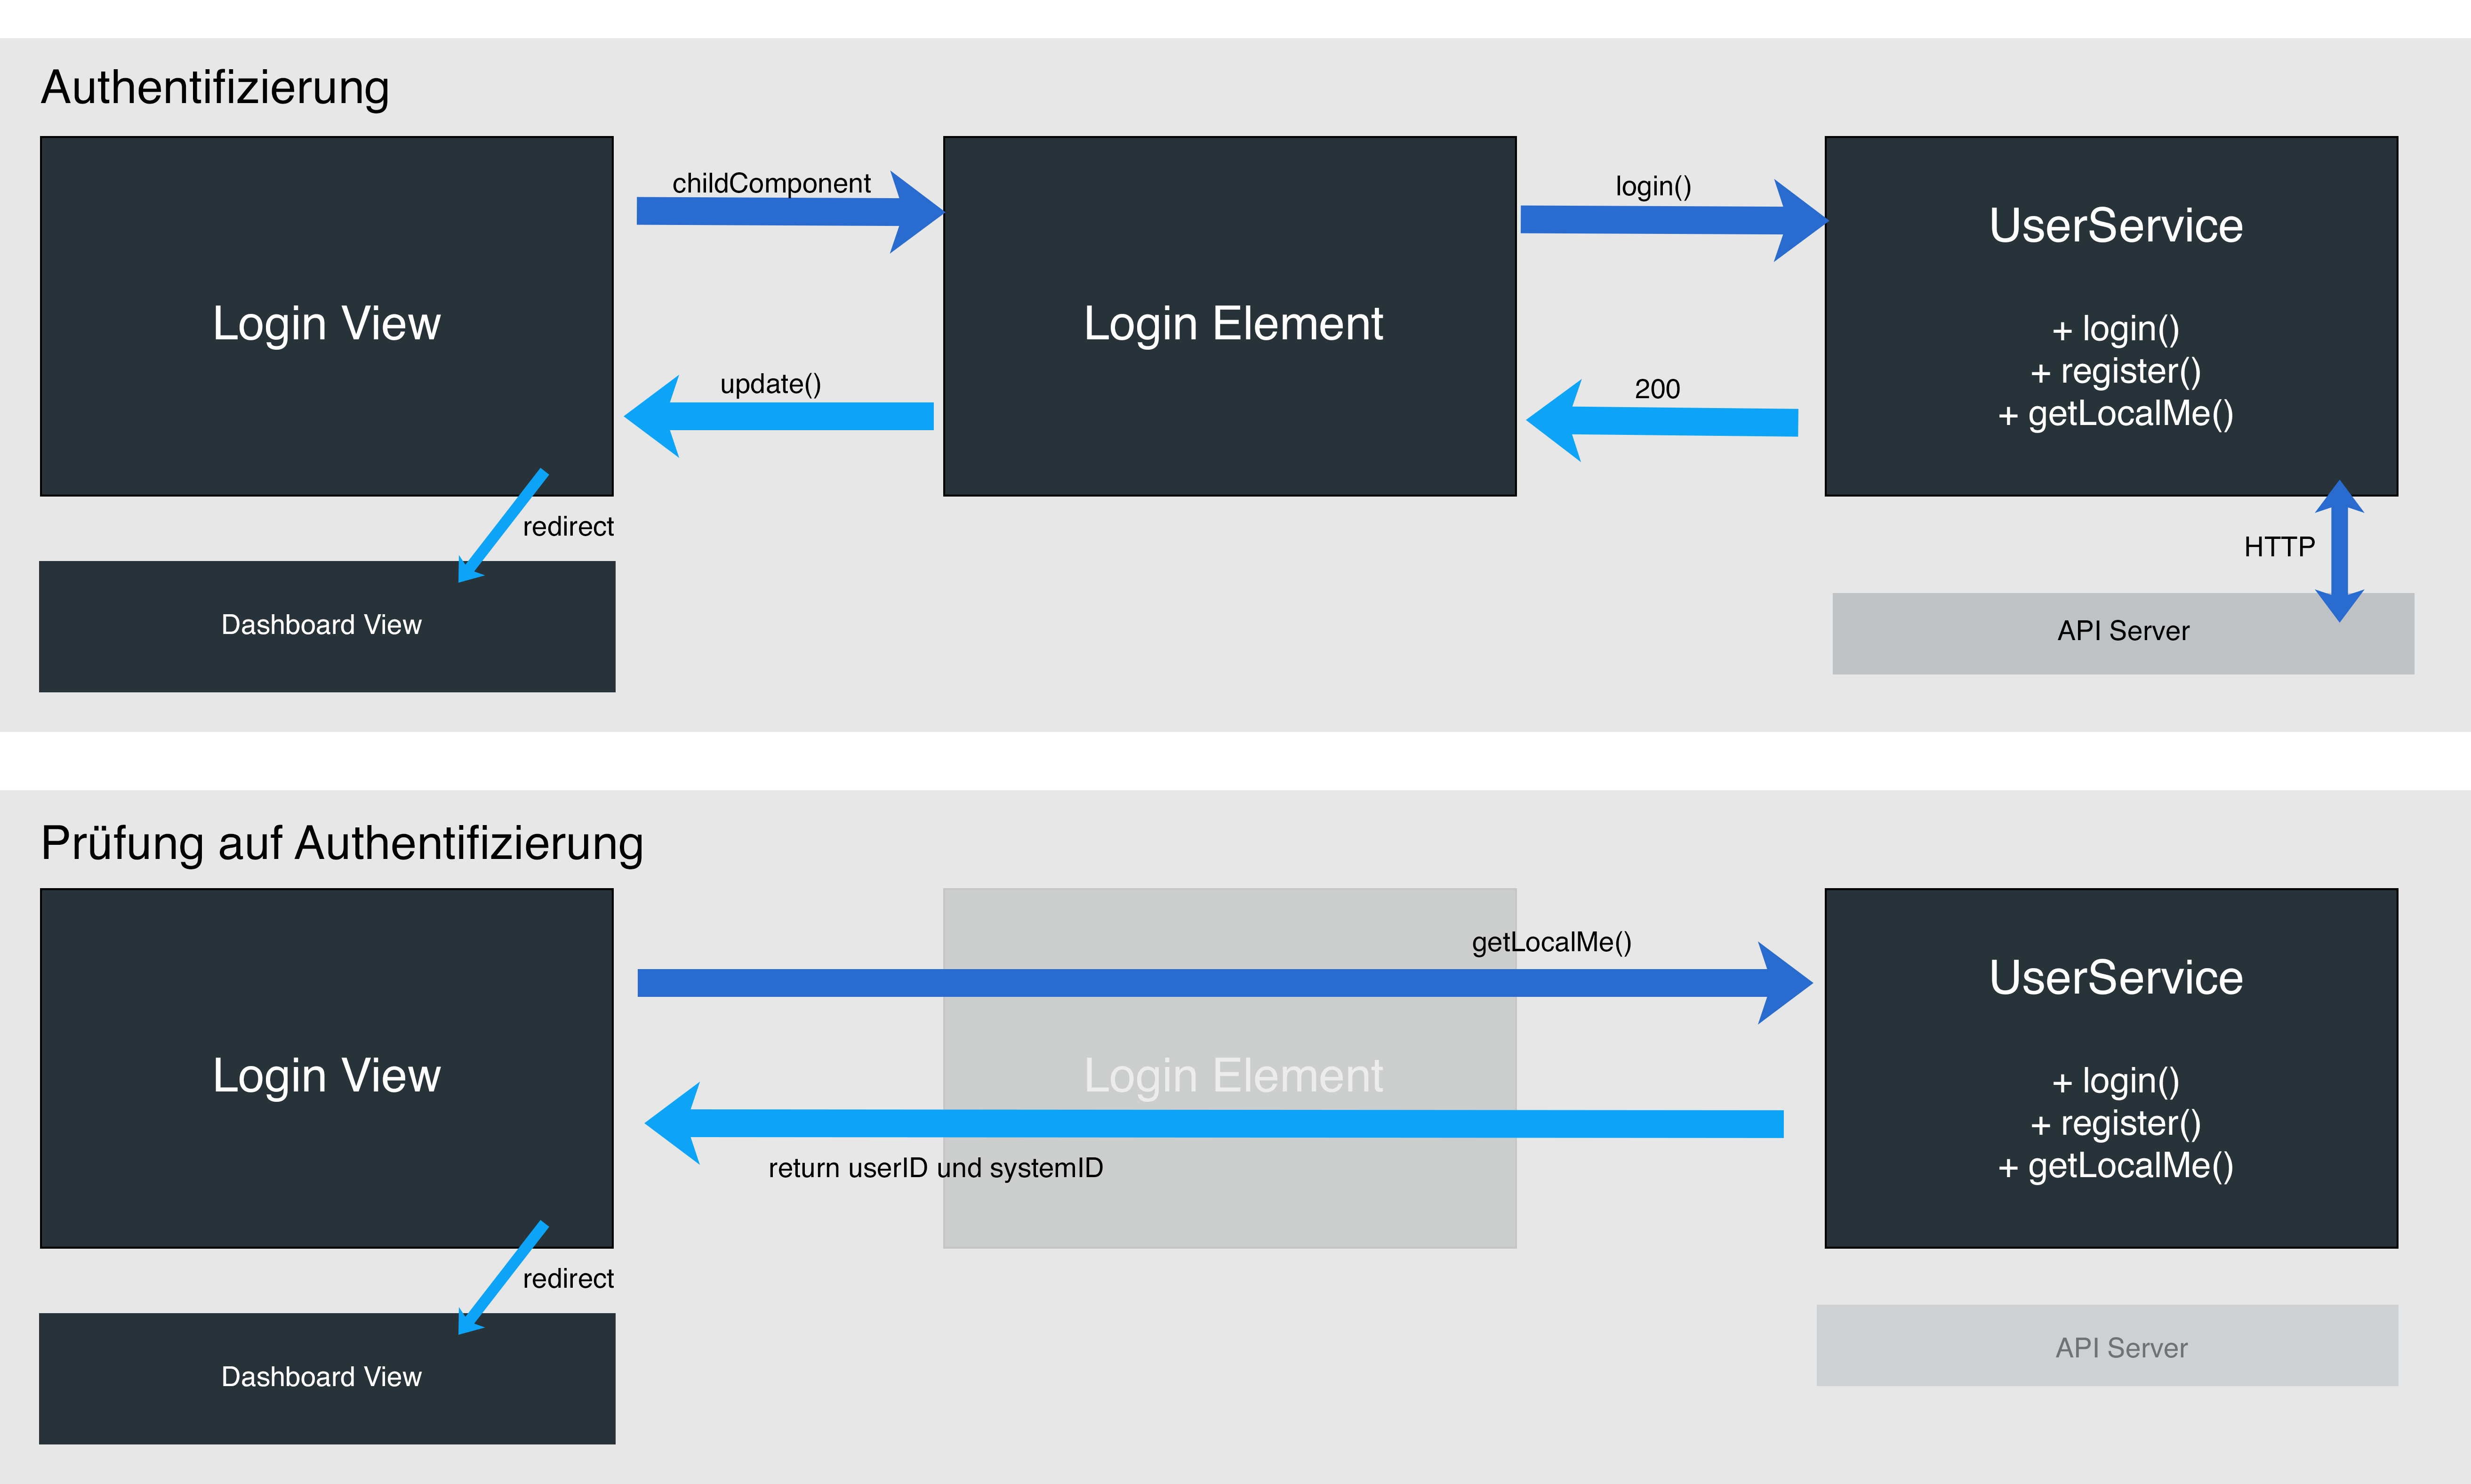
\includegraphics[width=\linewidth]{kapitel4/login.jpg}
 \caption{Login und User Service}
 \label{kapitel4/login}
\end{figure}
\vspace{0.3cm}

Anhand des spezifischen Ansatzes wurde eine Ansicht implementiert, in der sich Nutzer einloggen, registrieren und damit gegenüber der Applikation authentifizieren können.
Der \ac{API}-Server gibt dabei einen cookie-basierten Ansatz für die Authentifizierung vor. Der Login Ablauf wird in Abbildung \ref{kapitel4/login} veranschaulicht.
Zunächst wird die \emph{Login View} geladen, welche das \emph{Login Element} als Kind-Komponente enthält.
In dieser sind die nötigen Eingabefelder sowie die Anbindung an den \emph{User Service} implementiert.
Der \emph{User Service} bedient die Login und Register Schnittstelle des \ac{API}-Servers.
Nach erfolgreichem Login returniert der Server einen Statuscode von 200 (OK), welcher vom Service an das \emph{Login Element} propagiert wird.
Das \emph{Login Element} antwortet der \emph{Login View} mit einem Update Event, welche daraufhin zur \emph{Dashboard View} weiterleitet.

In der Implementierung des \emph{User Services}, siehe Anhang \ref{UserService}, werden innerhalb des Login- und Registriervorgangs
sowohl eine ID als auch der Name des Nutzers im Localstorage des Browsers persistiert.
Dies geschieht sehr elegant mithilfe des Variablen Decorators \emph{angular2-localstorage} \cite{marcj95:online}.
Die zu persistierenden Variablen werden mit \emph{@Localstorage} dekoriert, wodurch schreibender Variablenzugriff eine Persistierung auslöst.
Bei Lesezugriff auf die Variable werden zunächst Daten aus dem Localstorage geladen.
Interesant hierbei ist, dass selbst komplexe Objektstrukturen durch den Decorator zunächst serialisiert werden, um sie überhaupt im Localstorage speichern zu können.

Zum Zeitpunkt der \emph{Login View} Instanziierung wird der Localstorage im \emph{User Service} über die Funktion \emph{getLocalMe} ausgelesen.
Dies ermöglicht es Nutzer direkt zum Dashboard zu leiten, sollten diese bereits eingeloggt sein.
Zusätzlich ist ein globaler \emph{HTTP-Interceptor} implementiert, welcher bei jedem ausgehenden Request der Anwendung prüft, ob das zuvor gesetzte Cookie noch Gültigkeit besitzt.
Sollte eine Route des \ac{API}-Servers, welche Authentifizierung erfordert, einen Statuscode 401 (Unauthorized) liefern,
fängt der \emph{HTTP-Interceptor} den Fehler und leitet zur \emph{Login View} zurück, um den Nutzer für eine erneute Authentifizierung aufzufordern.




\subsubsection{Meta Picker}

Mit der \emph{Meta Picker Komponente} ist ein spezifisches, jedoch innerhalb der Anwendung wiederverwendbares Element implementiert, um Daten einer View hinsichtlich Applikationen und eines Zeitintervalls filtern zu können.
Diese Komponente findet derzeit Verwendung in der Metrik, Graphen und Traces Sektion. Wird eine Applikation beziehungsweise ein Zeitinterval über den Picker definiert,
wird diese Auswahl im Localstorage des Browsers persistiert und bei nachfolgenden Instanziierungen der Komponente zunächst aus dem Storage geladen und erneut ausgewählt.
Die Persistierung erfolgt hier ebenfalls über den Dekorator \emph{angular2-localstorage},
welcher bereits in der Implementierung \ref{Login-und-Authentifikation} Login und Authentifikation Verwendung fand.
Listing \ref{meta-picker-example} zeigt ein Verwendungsbeispiel der \emph{Meta Picker Komponente}.
Die binäre Option \emph{hideApplikation} versteckt das Auswahlfeld der Applikationen. Dies wird für die Graph Sektion benötigt,
da innerhalb dieser View das Zusammenspiel der einzelnen Services dargestellt wird und daher lediglich eine Filterung nach Zeit relevant ist.
Über die Funktion \emph{metaUpdate} werden Updates der Komponente abonniert. Wird eine Auswahl der Applikation oder des Zeitintervalls getätigt,
so propagiert der \emph{Meta Picker} ein Update an die äußere Eltern-Komponente. Die Variable \emph{\$event} beinhaltet dabei die vom Nutzer neu gesetzten Parameter.


\lstinputlisting[language=HTML,label=meta-picker-example,caption=Verwendungsbeispiel Meta Picker]{kapitel4/metapicker-example.html}


\begin{figure}[hptb]
 \centering
 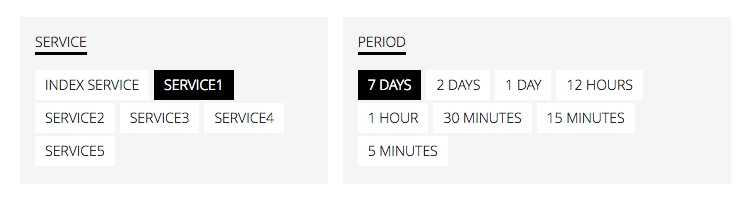
\includegraphics[width=0.8\linewidth]{kapitel4/metapicker.jpg}
 \caption{Meta Picker}
 \label{metapicker}
\end{figure}
\vspace{0.3cm}


\subsubsection{Traces}

Mithilfe der Traces Sektion werden serviceübergreifende Requests in Relation zur Zeit in einem Gantt Chart dargestellt.
Anhand der Visualisierung soll es für Anwendungsentwickler möglich sein, Verzögerungen oder Fehler im Aufrufstapel (Call Stack) identifizieren zu können.
Für die Umsetzung des Gantt Charts lag es zunächst nahe, eine bestehende Bibliothek zu verwenden.
Allerdings konnte keines der untersuchten Bibliotheken den Funktionsumfang bezüglich der Anforderungsanalyse abdecken.
Konfigurationsaufwand, Größe der Bibliothek und die Möglichkeit das Diagramm auch auf mobilen Geräten nutzen zu können, waren für die Untersuchung ausschlaggebende Kriterien.
Mit \emph{ng2-simplegantt} wurde daher eine eigene sehr vereinfachte Implementierung eines Gantt Diagramms, entsprechend dem generischen Ansatz, vorgenommen.

Die Daten werden zunächst über den anwendungsspezifischen Trace Service vom API-Server erfragt und anschließend innerhalb der ebenfalls spezifisch entwickelten \emph{Trace Komponente}
für die Darstellung in \emph{ng2-simplegantt} aufbereitet.
Bei der Implementierung der generischen Komponente wurde auf die Verwendung von absoluten Pixelwerten weitestgehend verzichtet.
Abstände und Positionen werden mithilfe von relativen Prozentwerten ausgedrückt. Dadurch ist die Komponente responsive und kann
ohne scriptbasierte rechenintensive Kalkulationen anhand der Bildschirmbreite auf Mobilgeräten verwendet werden.

\begin{itemize}
  \item{github.com/michaelknoch/ng2-simplegantt}
\end{itemize}

\subsubsection{Bibliothek Interfaces}

In \projectname{} werden die externen Bibliotheken \emph{Chart.js} und \emph{Cytoscape.js} verwendet.
Für deren Nutzung sind Interfaces in Form von Komponenten implementiert.
Dies bedeutet, dass Instanzen von Chart.js und Cytoscape.js nicht anhand globaler \ac{DOM} Zugriffe (Listing \ref{component-interface-1}),
sondern durch Angular Komponenten realisiert werden.


\paragraph{Chart.js} ist eine Bibliothek für das Zeichnen komplexer Diagramme.
Es wird in \projectname{} hauptsächlich für die Visualisierung der Daten für die Metrik Sektion verwendet.
Chart.js ist responsive implementiert, das heißt die Charts können sowohl für den Desktop
als auch für die Mobile Applikation verwendet werden \cite{Chart80:online}.

\vspace{0.3cm}
\lstinputlisting[language=JavaScript,label=component-interface-1,caption=Chart.js ohne Komponenten Interface]{kapitel4/chartjs-oldschool.js}

\lstinputlisting[language=JavaScript,label=component-interface-2,caption=Chart.js mit Komponenten Interface]{kapitel4/chartjs-new.js}
\vspace{0.3cm}
In Listing \ref{component-interface-2} wird die Nutzung des Komponenten Interface \emph{ng2-charts} verdeutlicht.
Daten- und Konfigurationsobjekte werden über den \emph{@Input} Kanal der Komponente von außen eingespeist.
Dadurch wird die Aggregation der Daten aus der Komponente heraus abstrahiert und es entsteht keine Ahängigkeit zu einem API-Service.
Die Komponente wird von Valor Software entwickelt und steht quelloffen unter der MIT Lizenz zur Verfügung \cite{valor6:online}.

Die Komponente erweist sich als sehr hilfreich, da das Chart bereits durch die simple Verwendung des Komponenten-Selektors (base-chart) instanziiert werden kann.
Des Weiteren werden die zu visualisierenden Daten sowie ein optionales Konfigurationsobjekt über den Selektor an die Komponenten übergeben.
Ändert sich das Datenobjekt, wird das Chart automatisch aktualisiert.



\paragraph{Cytoscape.js}
ist eine Bibliothek zur Visualisierung und Analyse komplexer Netzwerke.
Diese findet in \projectname{} Verwendung in der Implementierung der Graphen-Sektion,
in welcher Interaktionen zwischen Services visualisiert werden.
Um eine mit ng2-charts vergleichbar bequeme Nutzung der Graphen-Bibliothek zu ermöglichen,
wurde eine eigene Interface-Komponente entwickelt und open source auf Github veröffentlicht.

\begin{itemize}
  \item{github.com/michaelknoch/ng2-cytoscape}
\end{itemize}

\lstinputlisting[language=JavaScript,label=ng2-cytoscape,caption=ng2-cytoscape Implementierung]{kapitel4/ng2-cytoscape.ts}

\noindent Listing \ref{ng2-cytoscape} beinhaltet die Implementierung von ng2-cytoscape.
Um Übersicht gewährleisten zu können, wird für die Implementierung irrelevanter Inhalt einiger Konfigurationsobjekte mit (...) abgekürzt.

Bei der Instanziierung der Komponente werden erneut Daten und Konfigurationen über den Input Kanal von außen
in den Code der Komponente eingeschleust. Interessant hierbei ist,
dass lediglich das Datenobjekt \emph{elements} für die Nutzung der Komponente erforderlich ist.
Die Zuweisung der übrigen Variablen ist optional, da sie innerhalb des Konstruktors mit vorgegebenen Objekten initialisiert werden, sofern sie nicht bereits von außen definiert wurden.
Dadurch kann die Komponente bereits ohne eine ausgiebige Studie der Dokumentation verwendet und dennoch, falls verlangt, individuell konfiguriert werden.

Durch die Implementierung des \emph{onChanges} Interfaces und damit der Funktion \emph{ngOnChanges} wird sichergestellt,
dass der Graph neu gezeichnet wird, sobald sich Daten, welche mit \emph{@Input} dekoriert wurden, ändern.
Cytoscape.js erwartet für den Rendervorgang ein jQuery Element, auf welches die Funktion cytoscape({..})
mit den zuvor eingeschleusten Daten- und Konfigurationsobjekten angewandt wird.
Durch die Verwendung von \emph{ElementRef} aus dem Core von Angular, kann eine globale \ac{DOM} Selektion anhand von IDs oder Klassen vermieden werden, da \emph{elementRef.nativeElement} eine Referenz auf das native \ac{DOM} Objekt beinhaltet.

\subsubsection{Touch ID Komponente}

Abbildung \ref{touchidmock} zeigt die Touch ID Komponente, welche anhand des spezifischen Ansatzes für die mobile App implementiert wurde.
Mithilfe des Touch ID Fingerabdrucksensors kann nicht nur das Telefon selbst entsperrt werden,
der Fingerabdruck eines Anwenders kann auch innerhalb von mobilen Anwendungen als Authentifizierungsmittel genutzt werden.
In Sektion \ref{Login-und-Authentifikation} wurde eine Authentifizierung mittels Mail und Passwort erläutert,
dieser Schritt ist nach wie vor erforderlich. Durch Touch ID wurde eine weitere Sicherheitsschicht unabhängig der cookie-basierten Authentifizierung über den API-Server implementiert.
Sobald ein Nutzer durch seine Legitimationen eingeloggt wurde, ist für jeden weiteren Start der Anwendung kein erneuter Login erforderlich.
Durch den Einsatz von Touch ID erscheint jedoch beim Öffnen der App eine Aufforderung, die Identität durch den Fingerabdruck zu verifizieren, um womöglich sensible Anwendungsdaten vor unautorisierten Zugriff zu schützen.
Die Implementierung, welche in Listing \ref{touchid} zu sehen ist, basiert dabei auf dem Cordova Plugin \emph{cordova-plugin-touch-id} \cite{EddyV87:online}.

\vspace{0.3cm}
\begin{figure}[h!]
 \centering
 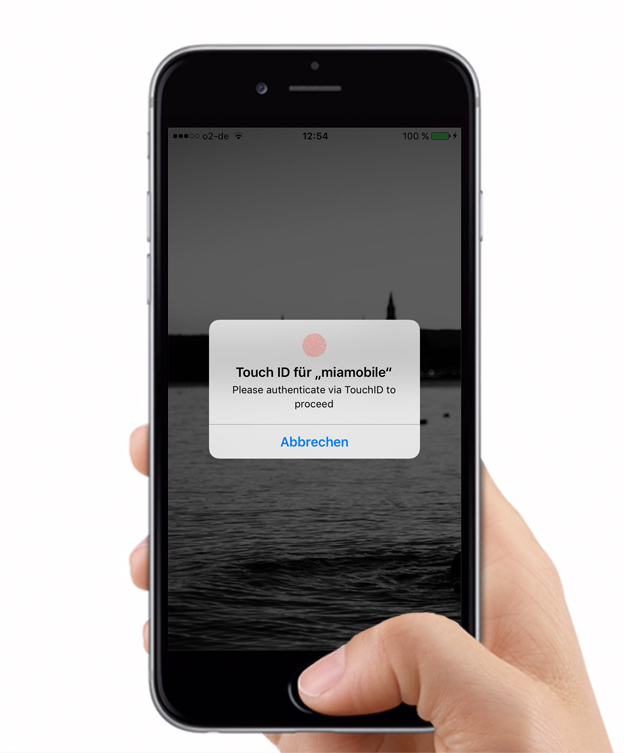
\includegraphics[width=0.5\linewidth]{kapitel4/touchid-mock.jpg}
 \caption{Touch ID Komponente}
 \label{touchidmock}
\end{figure}

Die Touch ID Komponente wird in die äußerste Komponente der mobilen Anwendung eingebunden,
dies ermöglicht, ein sperrendes Overlay über die Anwendung legen zu können, unabhängig auf welcher
View sich ein Nutzer gerade befindet. Die Komponente beinhaltet eine boolesche Variable \emph{lock}
welche den Status des Overlays definiert. Der Wert der Variable wird bei Aktivierung der App durch das Event \emph{platform.resume}
verändert (Zeile 18), insofern das mobile Gerät Touch ID unterstützt (Zeile 15) und der Nutzer eingeloggt ist (Zeile 17).
Das in Abbildung \ref{touchidmock} dargestellte Szenario erscheint, die Anwendung ist durch das Overlay blockiert und der Nutzer wird aufgefordert sich über seinen Fingerabdruck auszuweisen.
Bei Erfolg wird die \emph{lock} innerhalb des Events \emph{touchid.authenticate} (Zeile 19) erneut gesetzt.
Das Overlay verschwindet und die Anwendung ist damit entsperrt. Mit dem Zugriff auf \emph{ngZone.run} (Zeile 21) wird eine Angular Change Detection manuell ausgelöst, da der Change Detection Vorgang nicht automatisch durch \emph{touchid.authenticate} ausgelöst wird.

Das Overlay selbst besteht aus einem \ac{HTML} Element (Zeile 8), welches in Abhängigkeit der Variable \emph{lock} die Klasse \emph{active} erhält.
Innerhalb von Listing \ref{touchid-style} ist die Visualisierung des Template Elements in Form von \ac{SASS} implementiert.
Durch die Verwendung von \emph{position: fixed} wird gewährleistet, dass das Overlay unabhängig von relativen Containern und Scrollpositionen innerhalb der Anwendung zu jeder Situation den Inhalt komplett verdecken kann.



\lstinputlisting[language=Javascript,label=touchid,caption=Touch ID Implementierung]{kapitel4/touchid.ts}

\lstinputlisting[language=Javascript,label=touchid-style,caption=Touch ID Overlay \ac{SASS}]{kapitel4/touchid.sass}



\newpage
\section{Komponentenverteilung}

\subsection{Verteilungsinfrastruktur}

Es wird eine Infrastruktur benötigt, um Komponenten projektübergreifend verteilen zu können.
Möglich wäre die Konfiguration von Symlinks des lokalen Dateisystems, um Komponenten in das Angular,
sowie Ionic Projekt zu integrieren. Symlinks lassen sich allerdings nicht versionieren, daher würde
für jeden neuen Entwickler ein komplexer initialer Konfigurationsaufwand entstehen.
Des Weiteren sollen Komponenten nicht nur innerhalb der Ionic App,
sondern in vielen weiteren auf Angular 2 basierenden Projekten wiederverwendet werden können.
Eine Komponente oder ein Paket diverser Komponenten soll veröffentlicht, aktuell
gehalten und von Anwendungsentwicklern genutzt werden können.

Es liegt nahe dieses Problem mithilfe eines Paketmanagers zu lösen. Angular und Ionic verwenden für das Management
ihrer Kern-Abhängigkeiten \ac{NPM}.
Open Source Pakete können damit kostenfrei veröffentlicht und aktualisiert werden.
Da \projectname{} open source entwickelt wird,
reicht ein kostenfreier Basis-Account für die Verteilung der Awendungs-Komponenten völlig aus.

Es wäre denkbar, jede Komponente über ein eigenes \ac{NPM} Paket zu veröffentlichen.
Allerdings würde dies nicht nur den Veröffentlichungs- und Update-Mechanismus erschweren,
sondern würde auch eine aufwändige Definition von Modulabhängigkeiten bedeuten.
Um die Komplexität der Infrastruktur nicht unnötig zu erhöhen,
werden Komponenten, welche anhand des spezifischen Ansatzes entwickelt werden,
gemeinsam innerhalb eines \ac{NPM} Moduls \emph{(mia-distributed)} verteilt.
Dadurch können alle spezifischen Abhängigkeiten innerhalb eines Pakets aufgelöst werden.
Generische Komponenten werden jeweils eigenständig veröffentlicht und als Abhängigkeiten von \emph {mia-distributed} deklariert.
So wird sichergestellt, dass generisch entwickelte Abhängigkeiten beim installieren von \emph{mia-distributed}
ebenfalls geladen und installiert werden und diese dennoch problemlos von dritten verwendet werden können.

\subsection{Vorbereitung und Veröffentlichung}

Die zu verteilenden Komponenten sind in Typescript geschrieben,
daher müssen sie entweder im Zielprojekt in die Transpilierung mit einbezogen werden,
oder bereits vor der Verteilung transpiliert und damit als JavaScript Paket veröffentlicht werden.
Interessant hierbei sind die Optionen \emph{sourceMap} und \emph{declaration} des Typescript Transpilers.
Sind diese aktiviert, werden neben den transpilierten .js Javascript Dateien jeweils d.ts und .map Dateien abgelegt.

\subsubsection{Declaration(d.ts)}

Eine d.ts Datei wird als TypeScript Declaration File bezeichnet.
Es beschreibt Implementierungen, welche in JavaScript geschrieben sind oder von TypeScript zu JavaScript transpiliert wurden.
Das Declaration File ermöglicht die Verwendung von JavaScript Code, beispielsweise einer externen Bibliothek,
innerhalb eines TypeScript Projekts. Das Declaration File fungiert dabei als Typescript Interface
für die JavaScript Implementierung und gewährleistet statische Typisierung
und Autovervollständigung in unterstützenden IDEs.

Im TypeScript Transpilierungsprozess können Declaration Files mithilfe der Option \emph{declaration} generiert werden.
Für viele populäre JavaScript Bibliotheken wurden bereits Declaration Files von der Community oder von dem ursprünglichen Autor nachgeliefert.
In \projectname{} werden Declaration Dateien im Transpilierungsprozess generiert und mit der Komponente verteilt,
damit Typen und Schnittstellen der Komponenten im Ionic Projekt verwendet werden können \cite[471]{EssentialTS}.


\subsubsection{SourceMap (.map)}
Durch die Verwendung von *-to-JavaScript Transpilern und Minifizierungstools ensteht ein Problem, welches SourceMaps zu lösen versuchen.
Der zur Entwicklungszeit geschriebene Code ist nicht der selbe, welcher zur Laufzeit im Browser ausgeführt wird, da dieser transpiliert und womöglich minifiziert wurde.
Wenn nun Fehler der Applikation zur Laufzeit identifiziert werden, können diese nur erschwert auf den Ursprungscode abgebildet werden.
Der Typescript Transpiler beinhaltet einen SourceMaps Generator, welcher beim Transpilevorgang .map Dateien erzeugt,
welche dabei als Referenztabelle zwischen Quell- und Zielcode fungieren.
Wird die Entwicklerkonsole in einem Browser, welcher SourceMaps unerstützt, geöffnet, kann der ursprünglichen Code inspiziert werden.
SourceMaps werden in \projectname{} verwendet, um transpilierten Code während der Ausführung der Angular so wie Ionic Anwendung debuggen zu können
 \cite{Using97:online}.



\subsection{Verwendung im Ionic Projekt}
\ac{NPM} Module werden mit dem Befehl \emph{npm install} installiert.
Sie stehen im Projekt innerhalb der Node Modules zur Verfügung und können in das Projekt importiert und verwendet werden.

Bei der Wiederverwendung der entwickelten Komponenten im Ionic Projekt sind diverse Problemstellungen entstanden,
welche im Folgenden erläutert und gelöst werden.

\subsubsection{Absolute Asset Pfade}
\label{Absolute-Asset-Pfade}

Angular Komponenten enthalten Template Markup und \ac{CSS} Styling, welches entweder inline im Code der Komponente
definiert oder innerhalb externer \ac{HTML} und \ac{CSS} Dateien implementiert und über Dateipfade in der Komponente referenziert wird.
Abhängig von der Konfiguration der Komponente, des Modul Formats und des verwendeten Modul Loaders
können relative oder absolute Pfade zur Referenzierung der Markup und Style Assets angegeben werden.
In der Angular Applikation werden Module mithilfe von SystemJS geladen. Dies ermöglicht die Nutzung relativer Pfade.
Ionic hingegen liefert einen Deployment Prozess mithilfe von \emph{Browserify}, welcher eine absolute Referenz voraussetzt.
Die Verwendung von absoluten Pfaden ist keine Option, wenn Komponenten Codebase übergreifend Verwendung finden sollen,
da die Strukturen der beiden Applikationen komplett identisch sein müssten.
Eine einfache Lösung für dieses Problem wäre das Markup und Style nicht in externe Dateien auszulagern,
sondern diese innerhalb der Komponente zu definieren.
Dies führt allerdings schnell zu unübersichtlichen Komponenten,
wodurch deren Wartbarkeit und damit die Qualität der gesamten Anwendung drastisch abnehmen kann.

Um die Komponenten aus der Angular Applikation mit relativen Asset Pfaden nutzen zu können,
werden \ac{HTML} und \ac{CSS} Referenzen mithilfe des Moduls \emph{gulp-inline-ng2-template} noch vor der Verteilung zu Inline-Strings gewandelt \cite{ludoh30:online}.
Dadurch werden Konflikte bezüglich relativen und absoluten Referenz-Pfaden hinfällig.
Zudem wurde ein Pull Request in \emph{ionic-gulp-tasks} gestellt, welcher \emph{gulp-inline-ng2-template}
in den Ionic Build Prozess integriert und damit die Nutzung relativer Asset Pfade mit \emph{Browserify} ermöglicht.
Bisher wurde der Pull Request allerdings nicht gemerged, vermutlich weil diese Build Prozess Modifzierung die
Transpilierungsdauer einer Ionic App von zwei auf zehn Sekunden erhöht.
Das Ionic Team evaluiert derzeit Möglichkeiten für die Nutzung relativer Asset Pfade \cite{relat31:online}.

\subsubsection{Angular2-Localstorage Inkompatibilität}
In Abschnitt \ref{Login-und-Authentifikation} wurde die lokale persistierung der Nutzerdaten im Localstorage
des Browser anhand des \emph{angular2-localstorage} Decorators erläutert.
Der Decorator wird über den Bootstrap Prozess der Angular Applikation registriert,
dadurch werden Schreibzugriffe auf Variablen erfasst und Daten gespeichert.
Allerdings unterscheidet sich der Bootstrap einer Ionic Anwendung von dem einer Angular Applikation.
Es stellt sich heraus, dass \emph{angular2-localstorage} nicht ohne Weiteres im Ionic Projekt verwendet werden kann.
Da jedoch Funktionalität des \emph{User Services} und des \emph{Meta Pickers} auf dem Decorator aufbaut,
gilt es dieses Problem zu lösen.

Zuvor wurde in Abschnitt \ref{sec:services} erläutert, wie
Implementierungen von Services dynamisch ausgetauscht werden können.
Die Services, welche den problematischen Decorator beinhalten, werden also für die Ionic Anwendung neu geschrieben
und mithilfe eines Providers mit der ursprünglichen Implementierung ausgetauscht.
Statt die Variablen mit dem Storage Decorator zu persistieren, ist im neuen Service eine \emph{persistUser} Funktion implementiert, welche die erforderlichen Nutzerdaten nach
erfolgreichem Login- oder Registrierungsvorgang serialisiert und in den Localstorage speichert.
Durch einen manuellen Lesezugriff auf den Localstorage werden die Variablen innerhalb des Konstruktors initialisiert.
Um sicherzustellen, dass der Service die nötige Funktionalität vollständig abdeckt, implementieren beide Services ein Interface,
welches die erforderlichen Schnittstellen vorgibt. Das Interface ist in Listing \ref{userservice-interface} implementiert.

\vspace{0.3cm}

\lstinputlisting[language=Javascript,label=userservice-interface,caption=User Service Interface]{kapitel4/userservice-interface.ts}



\newpage
\section{Auslieferung}

Um die Auslieferung für die jeweiligen Plattformen zu ermöglichen,
sind im Rahmen des Projekts \projectname{} diverse Deployment Prozesse entstanden,
welche im Folgenden erläutert werden.

\subsection{Web}
\label{deployment-web}

Die Web-Applikation wird über die \ac{AWS} Instanz ausgeliefert, auf welcher sich auch der \ac{API}-Server befindet.
Aufgrund großer Unzufriedenheit mit der anfänglichen Ladezeit der Anwendung von nahezu 10 Sekunden wurde ein Deployment
Prozess konzipiert, welcher die Dauer des Ladevorgangs deutlich reduziert.
Ohne Optimierungen werden beim Start der Anwendungen 624 verschiedene Dateien geladen,
welche insgesamt eine Größe von 2,4MB aufweisen.
Dabei stellen Komponenten und Services der eigentlichen Implementierung nur einen Bruchteil der Menge dar.
Der Hauptteil besteht aus dem Angular 2 Kern und der Bibliothek RxJs, welche für den Betrieb von Angular benötigt wird.
Zunächst werden externe \ac{HTML} und \ac{CSS} Assets von Komponenten in
inline Strings umgewandelt und anschließend wird die ganze Applikation in einer \emph{app.bundle.js} Datei zusammengefasst.
Möglich wäre, den Code aus der resultierenden app.bundle.js zu minifizieren,
wodurch er weiter an Dateigröße verlieren würde. Da sich die Applikation \projectname{}
jedoch noch nicht in einem produktionsreifen Zustand befindet, wird Minifizierung zunächst ausgelassen.
Die 624 Dateirequests konnten auf 16 reduziert werden, wodurch die Applikation bereits nach 1,9
Sekunden vollständig geladen werden kann.
Die Menge der geladenen Daten wird aufgrund fehlender Minifizierung nahezu kaum reduziert.

\subsection{Desktop}

\subsubsection{Auslieferung}
Um die Ladezeit der Desktop-App ebenfalls gering zu halten, baut der Auslieferungsprozess der Electron-App
auf den in \ref{deployment-web} beschrieben Prozess der Webapplikation auf. Daher werden Applikationscode und die
Abhängigkeiten von Angular zunächst ebenfalls zu einer app.bundle.js Datei zusammengefasst.
Das Node Modul \emph{electron-packager} ermöglicht die Generierung der Electron-App für verschiedene Plattformen,
welche eigenständig ausgeführt werden kann.
Ein weiteres Node Modul \emph{electron-release} ermöglicht eine Veröffentlichung
der Anwendung innerhalb der Releases auf dem Github Repository.
Dort kann die App von Nutzern heruntergeladen und verwendet werden.

\subsubsection{Client Aktualisierung}
\label{client-updates}

Desktop Apps können entweder manuell durch Initivative der Nutzer oder durch
automatische Client Updates aktuell gehalten werden.
Electron bietet mit \emph{autoUpdater} eine Implementierung
von automatischen Updates im Hintergrund an.
Electron \emph{autoUpdater} ist dabei eine Schnittstelle, welche das \emph{Squirrel Framework}
für Automatisierungen von Windows und MacOS Anwendungen bedient.
Notwendig für die Hintergrundaktualisierung ist ein HTTP-Service, welcher beim Start der Anwendung mit der
aktuellen Version angefragt werden kann
und daraufhin einen Downloadpfad für ein eventuell verfügbares Update liefert.
Sollte kein Update zur Verfügung stehen, wird ein Statuscode 204 (No Content) geliefert.
Electron \emph{autoUpdater} lädt die neue App herunter, entpackt diese und tauscht den Webinhalt der Anwendung zur Laufzeit aus.
Wird die App nun neu gestartet, steht die neue Version zur Verfügung.

Im Ramen des Projekts \projectname{} wurde ein HTTP-Service für die
Verwendung von Electron \emph{autoUpdater} implementiert.
\begin{itemize}
\item github.com/michaelknoch/mia-electron-autoupdater-server
\end{itemize}

\subsubsection{Update Notifications}

Während der Updatevorgang einer Electron App im Main Kontext der
Anwendung stattfindet, ist der Render Prozess beziehungsweise der Angular Kontext unwissend über die aktuelle
Version der App sowie den Status des Updates. Um relevante Informationen für Nutzer innerhalb der Anwendung darstellen zu können,
müssen dem Render Kontext genannte Information bereitgestellt werden.
Daher wird Electrons \emph{IPC} Schnittstelle für einen asynchronen Austausch von Daten implementiert.

Beim Start der Anwendung wird zunächst die aktuelle Anwendungsversion innerhalb des Node Kontextes aus der Package.json der Desktop-Anwendung gelesen.
Anhand dieser Versionsummer wird gegen den HTTP-Service geprüft, ob ein Update vefügbar ist. Der Download des Updates beginnt bereits automatisch,
sobald der API-Endpoint einen Downloadpfad returniert.

Zeitgleich findet der Bootstrap Prozess der Angular Applikation im Render Prozess statt.
Ist dieser abgeschlossen, startet der \emph{IPC Service}, welcher bereits während seiner Instanziierung den
IPC Request ``version-request'' an den Node Kontext übermittelt.
Dieser antwortet daraufhin mit der zuvor ausgelesenen Version der Anwendung, welche im Angular Kontext wiederum als HTML5 Push Notification, siehe Abbildung \ref{kapitel4/update-push}, ausgegeben wird.

War der Download des Updates efolgreich, löst der Update Prozess das Event ``update-downloaded'' im Node Kontext aus,
welches durch IPC an den \emph{IPC Service} der Angular Applikation weitergeleitet wird. Erneut erscheint eine für den Nutzer bestimmte Notification, siehe Abbildung \ref{kapitel4/update-push}, welche auf Klick einen Restart der Applikation auslöst.
Dies ist mithilfe eines Klick Listeners realisiert, der dem Node Kontext das Event ``force-restart'' propagiert.
Daraufhin wird ``quitAndInstall'' über die \ac{API} des Updaters aufgerufen, wodurch die Applikation veranlasst wird, sich selbst zu beenden und in der neuen Version zu erscheinen.


\begin{figure}[h]
 \centering
  
\includegraphics[width=0.5\linewidth]{kapitel4/version-push.jpg}
 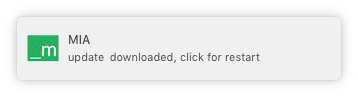
\includegraphics[width=0.5\linewidth]{kapitel4/update-push.jpg}
 \caption{Update Notifications}
 \label{kapitel4/update-push}
\end{figure}
\vspace{0.3cm}


\subsection{App}

Die iOS und Android App wird mithilfe der Ionic \ac{CLI} gebaut und muss daraufhin für den
jeweiligen App Store veröffentlicht werden. Der Build Prozess,
welcher durch den Befehl \emph{ionic build ios} und \emph{ionic build android} ausgeführt wird,
erstellt dabei die Applikation für die jeweilige Zielplattform.
Für die Veröffentlichung in den Stores ist zunächst die Freischaltung eines Entwickler Accounts erforderlich,
welche durch eine einmalige Zahlung von 25\$ für den Google Play Store beziehungsweise einer jährlichen Gebühr von 99\$
für den iOS App Store sowie einer Prüfung der Person oder des Unternehmens erfolgt.
